A ConvNeXt-Tiny iteratív tanításának eredményei négy lépésben először 1000 majd 5000 azután 10000 végül pedig 25000 képes halmazon. Ezelet a lépéseket 1k, 5k 10k 25k rövidítésekkel fogom jelölni.

%1K-----------------------------------------------------------------------------
\subsubsection{1k adathalmazon történő tanítás lépései ConvNeXt-Tiny modellen.}
  \begin{itemize} 
    \item Epoch 1/10 - train: 15/15 [00:04<00:00,  3.32it/s]
    \item Epoch 1: Train loss=4.7483, acc=0.0373 Val loss=4.2324, acc=0.1041
    \item Epoch 2/10 - train: 15/15 [00:03<00:00,  4.30it/s]
    \item Epoch 2: Train loss=3.3442, acc=0.3081 Val loss=3.5033, acc=0.2087
    \item Epoch 3/10 - train: 15/15 [00:03<00:00,  4.30it/s]
    \item Epoch 3: Train loss=1.4775, acc=0.6974 Val loss=3.0465, acc=0.2618
    \item Epoch 4/10 - train: 15/15 [00:03<00:00,  4.30it/s]
    \item Epoch 4: Train loss=0.4137, acc=0.9419 Val loss=2.8786, acc=0.2941
    \item Epoch 5/10 - train: 15/15 [00:03<00:00,  4.31it/s]
    \item Epoch 5: Train loss=0.1225, acc=0.9814 Val loss=2.9332, acc=0.2925
    \item Epoch 6/10 - train: 15/15 [00:03<00:00,  4.29it/s]
    \item Epoch 6: Train loss=0.0785, acc=0.9868 Val loss=2.9832, acc=0.2908
    \item Epoch 7/10 - train: 15/15 [00:03<00:00,  4.30it/s]
    \item Epoch 7: Train loss=0.0481, acc=0.9901 Val loss=3.0014, acc=0.2930
    \item Epoch 8/10 - train: 15/15 [00:03<00:00,  4.30it/s]
    \item Epoch 8: Train loss=0.0269, acc=0.9945 Val loss=2.8885, acc=0.3147
    \item Epoch 9/10 - train: 15/15 [00:03<00:00,  4.29it/s]
    \item Epoch 9: Train loss=0.0261, acc=0.9945 Val loss=2.9716, acc=0.2993
    \item Epoch 10/10 - train: 15/15 [00:03<00:00,  4.29it/s]
    \item Epoch 10: Train loss=0.0258, acc=0.9945 Val loss=2.9300, acc=0.3059
  \end{itemize}

\subsubsection{1k adathalmazon történő tanítás grafikonja ConvNeXt-Tiny modellen.}
  \begin{figure}[H]
    \centering
    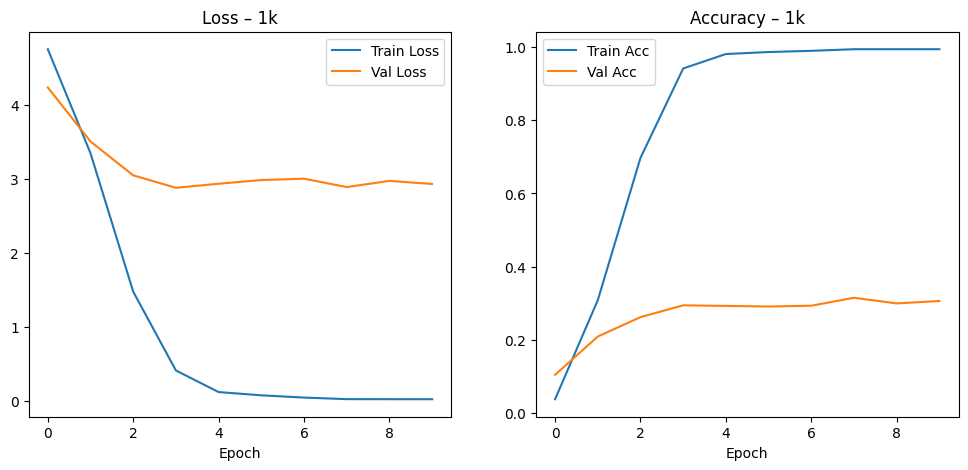
\includegraphics[width=1.0\textwidth]{images/phase03/phase03_ConvNeXt-Tiny_1K_learning_curve.png}
    \caption{1k adathalmazon történő tanítás grafikonja ConvNeXt-Tiny modellen.}
    \label{fig:phase03_ConvNeXt-Tiny_1K_learning_curve}
  \end{figure}

  \subsubsection{1k adathalmazon történő tanítás eredményei.}
    \begin{center}
      \begin{longtable}{l c}
      \caption{1k tanítás ConvNeXt-Tiny-en.} \label{tab:phase03_ConvNeXt-Tiny_1k} \\
      \toprule
      \textbf{Metrika} & \textbf{Érték} \\
      \midrule
      \endfirsthead
      \toprule
      \textbf{Metrika} & \textbf{Érték} \\
      \midrule
      \endhead
      Top-1 Accuracy & 0.3172 \\
      Top-5 Accuracy & 0.6230 \\
      Precision      & 0.3031 \\
      Recall         & 0.3453 \\
      F1-score       & 0.3026 \\
      Inference time & 25.45 sec \\
      \bottomrule
      \end{longtable}
    \end{center}

%5K-----------------------------------------------------------------------------
\subsubsection{5k adathalmazon történő tanítás lépései ConvNeXt-Tiny modellen.}
\begin{itemize} 
	\item Epoch 1/10 - train: 77/77 [00:17<00:00, 4.41it/s]
	\item Epoch 1: Train loss=3.2323, acc=0.2640 Val loss=2.2990, acc=0.3980
	\item Epoch 2/10 - train: 77/77 [00:17<00:00, 4.42it/s]
	\item Epoch 2: Train loss=1.3089, acc=0.6465 Val loss=2.0114, acc=0.4704
	\item Epoch 3/10 - train: 77/77 [00:17<00:00, 4.41it/s]
	\item Epoch 3: Train loss=0.4476, acc=0.8911 Val loss=2.1039, acc=0.4558
	\item Epoch 4/10 - train: 77/77 [00:17<00:00, 4.42it/s]
	\item Epoch 4: Train loss=0.1939, acc=0.9555 Val loss=2.0306, acc=0.4928
	\item Epoch 5/10 - train: 77/77 [00:17<00:00, 4.42it/s]
	\item Epoch 5: Train loss=0.1015, acc=0.9782 Val loss=2.1486, acc=0.4821
	\item Epoch 6/10 - train: 77/77 [00:17<00:00, 4.42it/s]
	\item Epoch 6: Train loss=0.0573, acc=0.9869 Val loss=2.0292, acc=0.5130
	\item Epoch 7/10 - train: 77/77 [00:17<00:00, 4.42it/s]
	\item Epoch 7: Train loss=0.0440, acc=0.9898 Val loss=2.1129, acc=0.5067
	\item Epoch 8/10 - train: 77/77 [00:17<00:00, 4.41it/s]
	\item Epoch 8: Train loss=0.0332, acc=0.9933 Val loss=2.0353, acc=0.5204
	\item Epoch 9/10 - train: 77/77 [00:17<00:00, 4.41it/s]
	\item Epoch 9: Train loss=0.0238, acc=0.9949 Val loss=2.3059, acc=0.4888
	\item Epoch 10/10 - train: 77/77 [00:17<00:00, 4.41it/s]
	\item Epoch 10: Train loss=0.0251, acc=0.9949 Val loss=2.0397, acc=0.5232
\end{itemize}

\subsubsection{5k adathalmazon történő tanítás grafikonja ConvNeXt-Tiny modellen.}
  \begin{figure}[H]
    \centering
    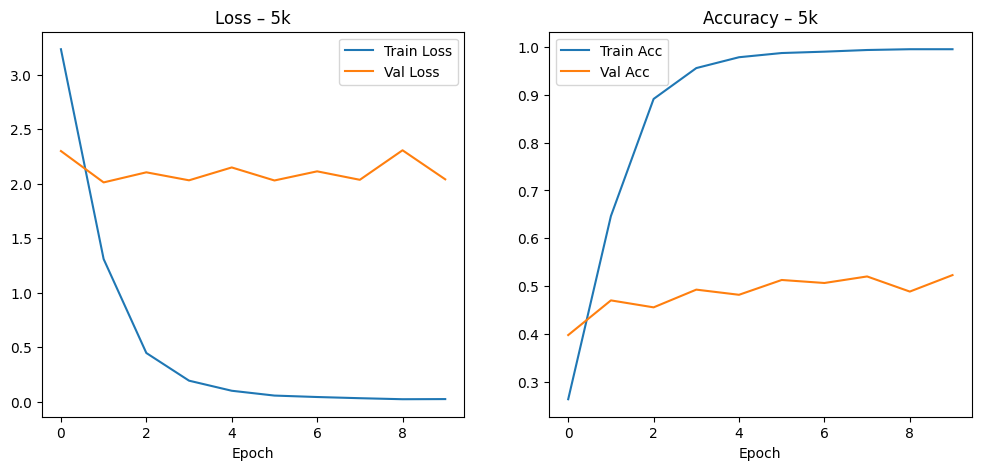
\includegraphics[width=1.0\textwidth]{images/phase03/phase03_ConvNeXt-Tiny_5K_learning_curve.png}
    \caption{5k adathalmazon történő tanítás grafikonja ConvNeXt-Tiny modellen.}
    \label{fig:phase03_ConvNeXt-Tiny_5K_learning_curve}
  \end{figure}

\subsubsection{5k adathalmazon történő tanítás eredményei.}
  \begin{center}
    \begin{longtable}{l c}
    \caption{5k tanítás ConvNeXt-Tiny-en.} \label{tab:phase03_ConvNeXt-Tiny_5k} \\
    \toprule
    \textbf{Metrika} & \textbf{Érték} \\
    \midrule
    \endfirsthead
    \toprule
    \textbf{Metrika} & \textbf{Érték} \\
    \midrule
    \endhead
    Top-1 Accuracy & 0.5305 \\
    Top-5 Accuracy & 0.8286 \\
    Precision      & 0.4896 \\
    Recall         & 0.5435 \\
    F1-score       & 0.4969 \\
    Inference time & 25.20 sec \\
    \bottomrule
    \end{longtable}
  \end{center}

%10K-----------------------------------------------------------------------------
\subsubsection{10k adathalmazon történő tanítás lépései ConvNeXt-Tiny modellen.}
  \begin{itemize} 
    \item Epoch 1/10 - train: 155/155 [00:34<00:00, 4.43it/s]
    \item Epoch 1: Train loss=2.6306, acc=0.3692 Val loss=1.9655, acc=0.4477
    \item Epoch 2/10 - train: 155/155 [00:34<00:00, 4.44it/s]
    \item Epoch 2: Train loss=1.1228, acc=0.6901 Val loss=1.7336, acc=0.5138
    \item Epoch 3/10 - train: 155/155 [00:34<00:00, 4.43it/s]
    \item Epoch 3: Train loss=0.4395, acc=0.8828 Val loss=1.8544, acc=0.5230
    \item Epoch 4/10 - train: 155/155 [00:34<00:00, 4.43it/s]
    \item Epoch 4: Train loss=0.1985, acc=0.9449 Val loss=1.9064, acc=0.5314
    \item Epoch 5/10 - train: 155/155 [00:34<00:00, 4.44it/s]
    \item Epoch 5: Train loss=0.1009, acc=0.9755 Val loss=2.0619, acc=0.5260
    \item Epoch 6/10 - train: 155/155 [00:34<00:00, 4.43it/s]
    \item Epoch 6: Train loss=0.0753, acc=0.9810 Val loss=1.9802, acc=0.5444
    \item Epoch 7/10 - train: 155/155 [00:34<00:00, 4.43it/s]
    \item Epoch 7: Train loss=0.0861, acc=0.9785 Val loss=2.0622, acc=0.5343
    \item Epoch 8/10 - train: 155/155 [00:34<00:00, 4.44it/s]
    \item Epoch 8: Train loss=0.0797, acc=0.9811 Val loss=2.0094, acc=0.5545
    \item Epoch 9/10 - train: 155/155 [00:34<00:00, 4.43it/s]
    \item Epoch 9: Train loss=0.0640, acc=0.9846 Val loss=2.2297, acc=0.5252
    \item Epoch 10/10 - train: 155/155 [00:34<00:00, 4.43it/s]
    \item Epoch 10: Train loss=0.0402, acc=0.9906 Val loss=2.2094, acc=0.5412
  \end{itemize}

\subsubsection{10k adathalmazon történő tanítás grafikonja ConvNeXt-Tiny modellen.}
  \begin{figure}[H]
    \centering
    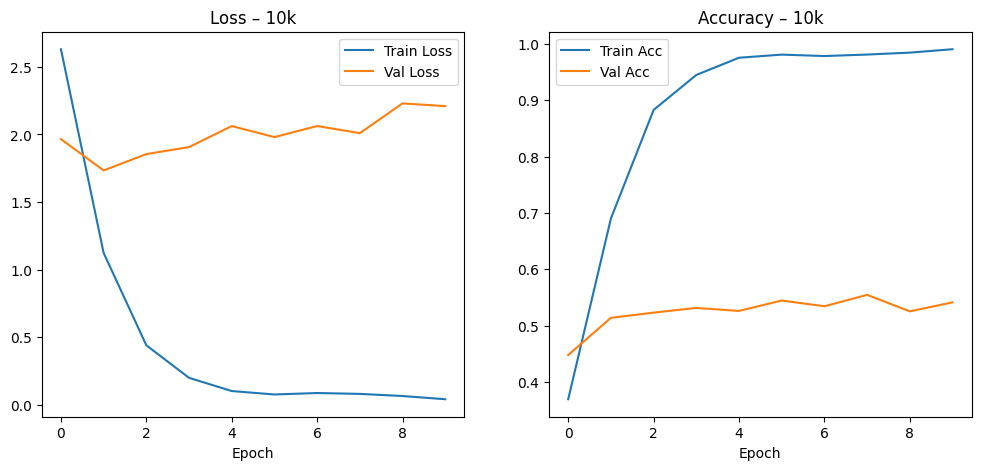
\includegraphics[width=1.0\textwidth]{images/phase03/phase03_ConvNeXt-Tiny_10K_learning_curve.png}
    \caption{10k adathalmazon történő tanítás grafikonja ConvNeXt-Tiny modellen.}
    \label{fig:phase03_ConvNeXt-Tiny_10K_learning_curve}
  \end{figure}

\subsubsection{10k adathalmazon történő tanítás eredményei.}
  \begin{center}
    \begin{longtable}{l c}
    \caption{10k tanítás ConvNeXt-Tiny-en.} \label{tab:phase03_ConvNeXt-Tiny_10k} \\
    \toprule
    \textbf{Metrika} & \textbf{Érték} \\
    \midrule
    \endfirsthead
    \toprule
    \textbf{Metrika} & \textbf{Érték} \\
    \midrule
    \endhead
    Top-1 Accuracy & 0.5416 \\
    Top-5 Accuracy & 0.8272 \\
    Precision      & 0.5079 \\
    Recall         & 0.5658 \\
    F1-score       & 0.5137 \\
    Inference time & 25.27 sec \\
    \bottomrule
    \end{longtable}
  \end{center}

%25K-----------------------------------------------------------------------------
\subsubsection{25k adathalmazon történő tanítás lépései ConvNeXt-Tiny modellen.}
  \begin{itemize} 
    \item Epoch 1/10 - train: 391/391 [01:27<00:00, 4.48it/s]
    \item Epoch 1: Train loss=2.1272, acc=0.4560 Val loss=1.7576, acc=0.5161
    \item Epoch 2/10 - train: 391/391 [01:27<00:00, 4.47it/s]
    \item Epoch 2: Train loss=0.9830, acc=0.7127 Val loss=1.5572, acc=0.5643
    \item Epoch 3/10 - train: 391/391 [01:27<00:00, 4.47it/s]
    \item Epoch 3: Train loss=0.4861, acc=0.8555 Val loss=1.6504, acc=0.5798
    \item Epoch 4/10 - train: 391/391 [01:27<00:00, 4.47it/s]
    \item Epoch 4: Train loss=0.2733, acc=0.9209 Val loss=1.7209, acc=0.5793
    \item Epoch 5/10 - train: 391/391 [01:27<00:00, 4.47it/s]
    \item Epoch 5: Train loss=0.1750, acc=0.9493 Val loss=2.0050, acc=0.5557
    \item Epoch 6/10 - train: 391/391 [01:27<00:00, 4.47it/s]
    \item Epoch 6: Train loss=0.1506, acc=0.9585 Val loss=1.8479, acc=0.5917
    \item Epoch 7/10 - train: 391/391 [01:27<00:00, 4.47it/s]
    \item Epoch 7: Train loss=0.1665, acc=0.9529 Val loss=2.2619, acc=0.5433
    \item Epoch 8/10 - train: 391/391 [01:27<00:00, 4.47it/s]
    \item Epoch 8: Train loss=0.1498, acc=0.9586 Val loss=2.1270, acc=0.5702
    \item Epoch 9/10 - train: 391/391 [01:27<00:00, 4.47it/s]
    \item Epoch 9: Train loss=0.1166, acc=0.9673 Val loss=2.2016, acc=0.5608
    \item Epoch 10/10 - train: 391/391 [01:27<00:00, 4.47it/s]
    \item Epoch 10: Train loss=0.1266, acc=0.9646 Val loss=2.2757, acc=0.5579
  \end{itemize}

\subsubsection{25k adathalmazon történő tanítás grafikonja ConvNeXt-Tiny modellen.}
  \begin{figure}[H]
    \centering
    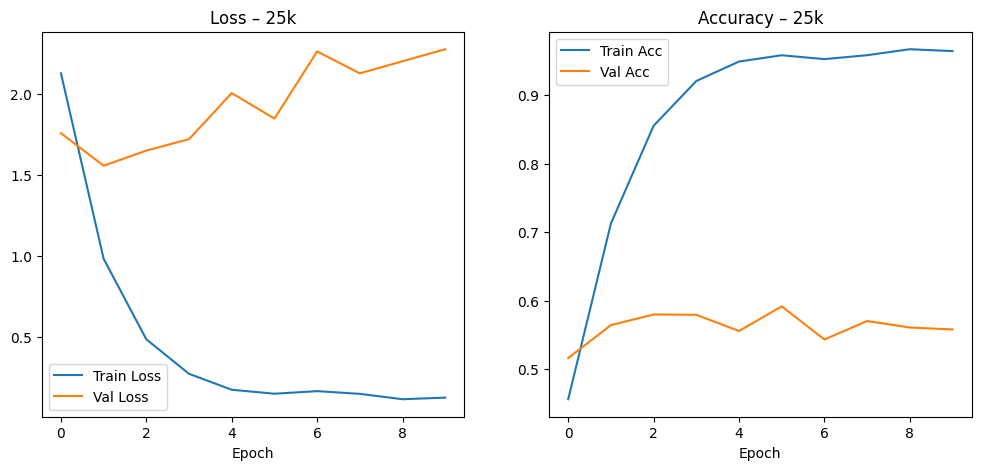
\includegraphics[width=1.0\textwidth]{images/phase03/phase03_ConvNeXt-Tiny_25K_learning_curve.png}
    \caption{25k adathalmazon történő tanítás grafikonja ConvNeXt-Tiny modellen.}
    \label{fig:phase03_ConvNeXt-Tiny_25K_learning_curve}
  \end{figure}

\subsubsection{25k adathalmazon történő tanítás eredményei.}
  \begin{center}
    \begin{longtable}{l c}
    \caption{25k tanítás ConvNeXt-Tiny-en.} \label{tab:phase03_ConvNeXt-Tiny_25k} \\
    \toprule
    \textbf{Metrika} & \textbf{Érték} \\
    \midrule
    \endfirsthead
    \toprule
    \textbf{Metrika} & \textbf{Érték} \\
    \midrule
    \endhead
    Top-1 Accuracy & 0.5687 \\
    Top-5 Accuracy & 0.8489 \\
    Precision      & 0.5602 \\
    Recall         & 0.6229 \\
    F1-score       & 0.5684 \\
    Inference time & 25.33 sec \\
    \bottomrule
    \end{longtable}
  \end{center}

\subsubsection{ConvNeXt-Tiny iteratív tanítás összefoglaló}
  \begin{center}
    \begin{longtable}{lllllll}
    \caption{Összehasonlító táblázat a ConvNeXt-Tiny iteratív tanításáról.}\label{tab:phase3_ConvNeXt-Tiny_summary_table}\\
    \toprule
    Minta & Top-1 & Top-5 & Precision & Recall & F1 & Time(s) \\
    \midrule
    \endfirsthead
    \toprule
    Minta & Top-1 & Top-5 & Precision & Recall & F1 & Time(s) \\
    \midrule
    \endhead
    1k & 0.3172 & 0.6230 & 0.3031 & 0.3453 & 0.3026 & 25.45 \\
    5k & 0.4757 & 0.7744 & 0.4532 & 0.5066 & 0.4602 & 25.31 \\
    10k & 0.5416 & 0.8272 & 0.5079 & 0.5658 & 0.5137 & 25.27 \\
    25k & 0.5687 & 0.8489 & 0.5602 & 0.6229 & 0.5684 & 25.33 \\
    \bottomrule
    \end{longtable}
  \end{center}
  
  \subsubsection{Összehasonlító grafikon a ConvNeXt-Tiny iteratív tanításáról.}
  \begin{figure}[H]
    \centering
    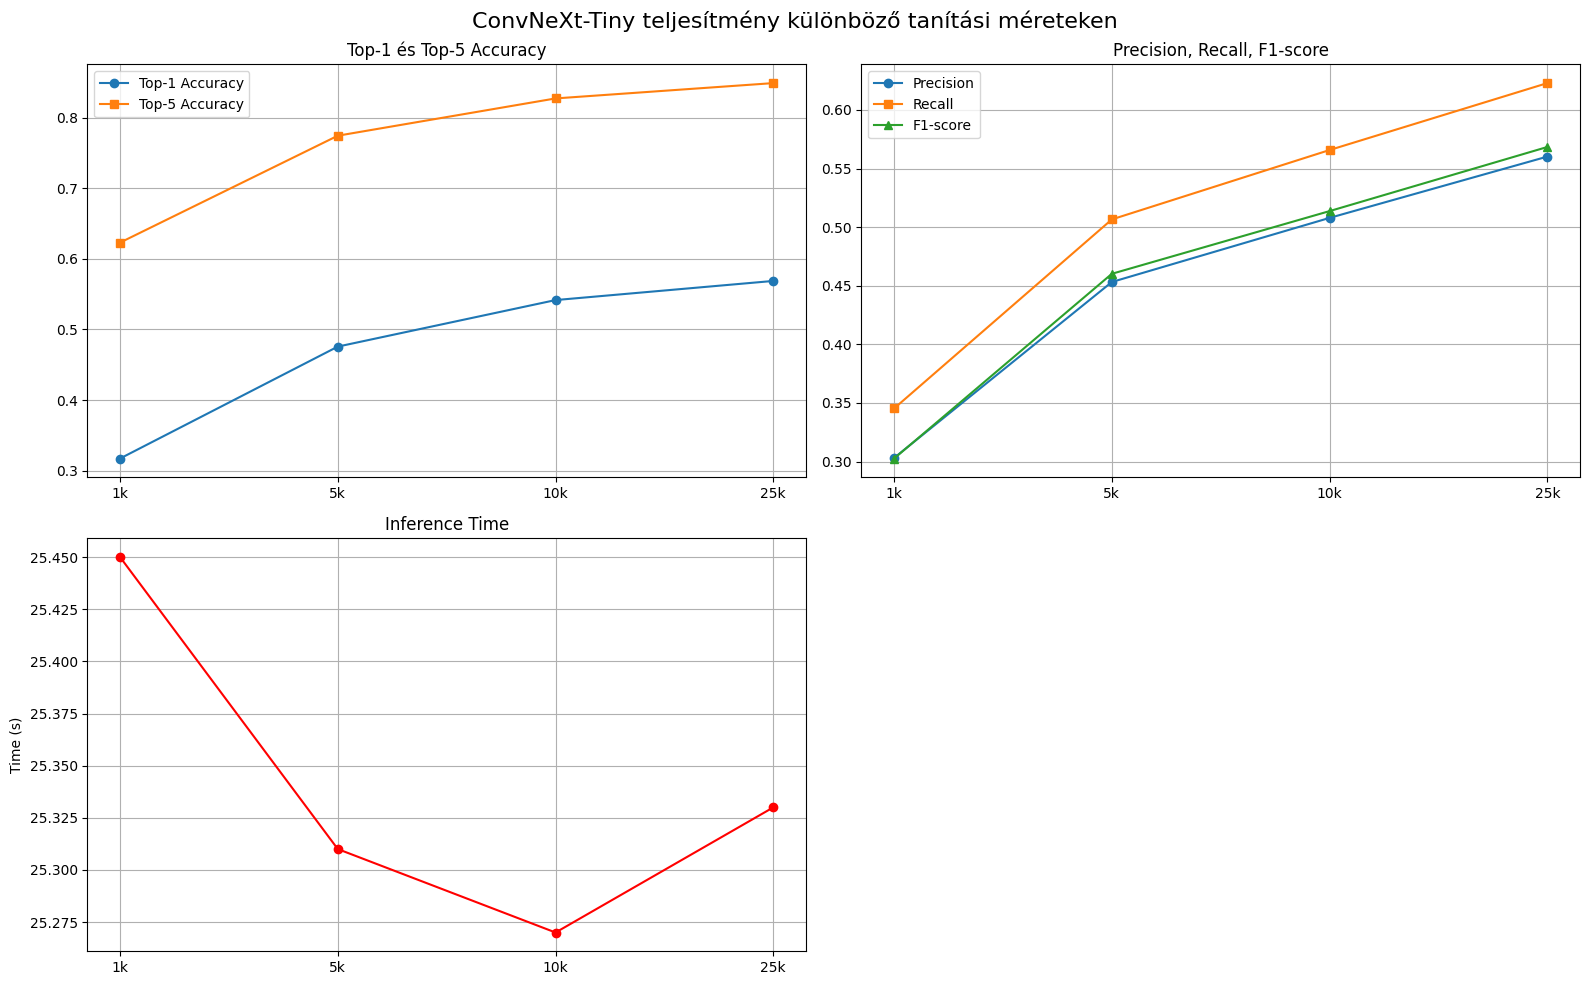
\includegraphics[width=1.0\textwidth]{images/phase03/phase03_ConvNeXt-Tiny_summary_curve.png}
    \caption{Összehasonlító grafikon a ConvNeXt-Tiny iteratív tanításáról.}
    \label{fig:phase03_ConvNeXt-Tiny_summary_curve}
  \end{figure}

  \subsubsection{Összehasonlító metrika grafikon a ConvNeXt-Tiny iteratív tanításáról.}
  \begin{figure}[H]
    \centering
    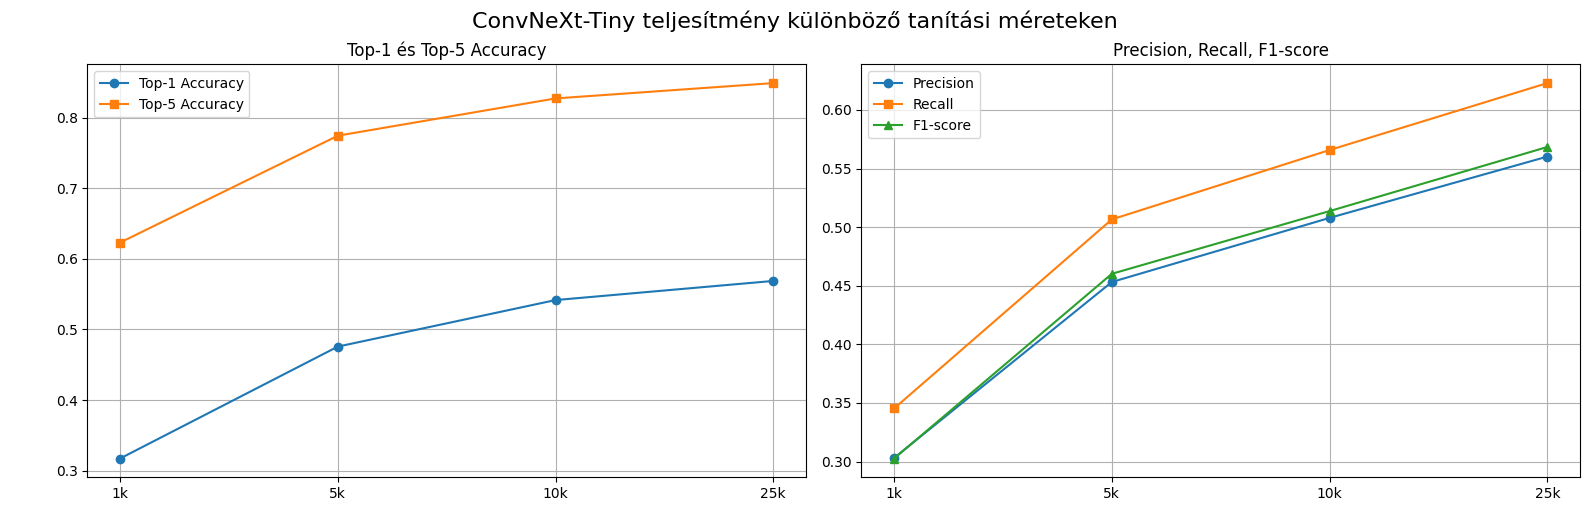
\includegraphics[width=1.0\textwidth]{images/phase03/phase03_ConvNeXt-Tiny_summary_curve_metrics.png}
    \caption{Összehasonlító metrika grafikon a ConvNeXt-Tiny iteratív tanításáról.}
    \label{fig:phase03_ConvNeXt-Tiny_summary_curve_metrics}
  \end{figure}

  \subsubsection{Összehasonlító idő grafikon a ConvNeXt-Tiny iteratív tanításáról.}
  \begin{figure}[H]
    \centering
    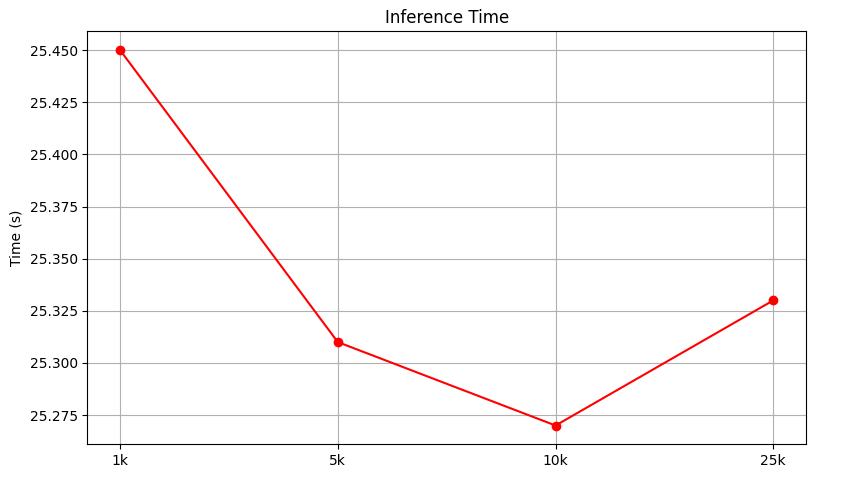
\includegraphics[width=1.0\textwidth]{images/phase03/phase03_ConvNeXt-Tiny_summary_curve_time.png}
    \caption{Összehasonlító idő grafikon a ConvNeXt-Tiny iteratív tanításáról.}
    \label{fig:phase03_ConvNeXt-Tiny_summary_curve_time}
  \end{figure}

  \subsubsection{Összehasonlító grafikon a ConvNeXt-Tiny iteratív tanításáról 10 EPOCH-on keresztül.}
  \begin{figure}[H]
    \centering
    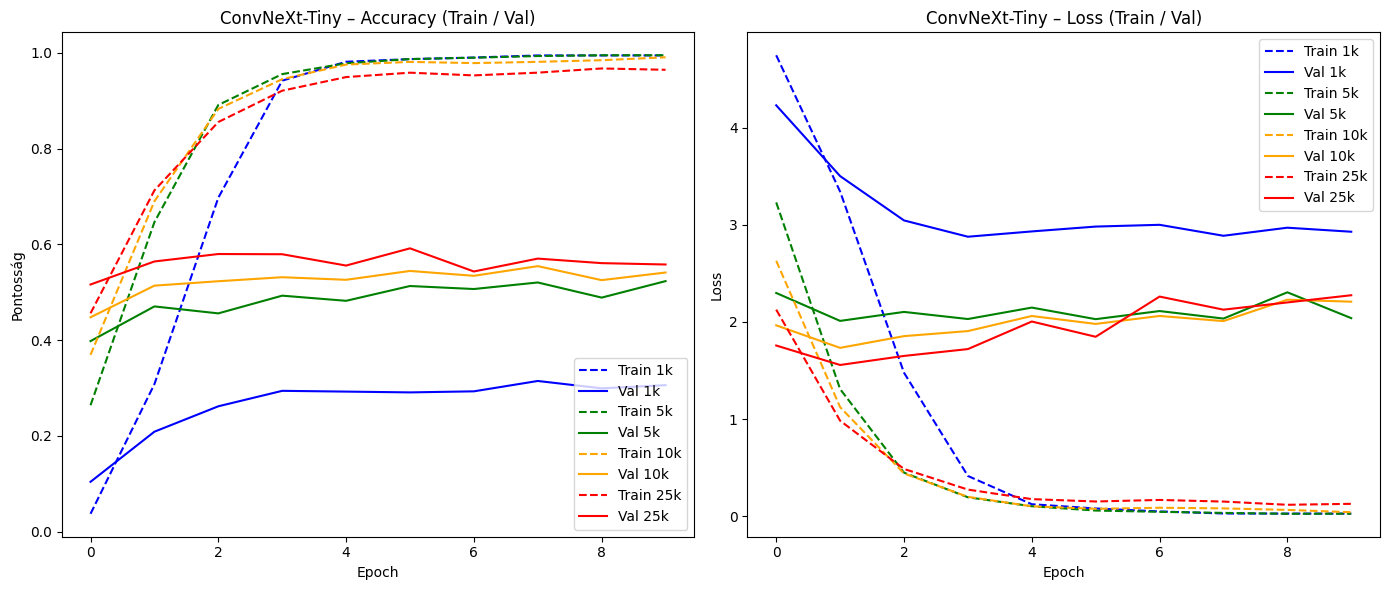
\includegraphics[width=1.0\textwidth]{images/phase03/phase03_ConvNeXt-Tiny_learning_summary_curve.png}
    \caption{Összehasonlító grafikon a ConvNeXt-Tiny iteratív tanításáról 10 EPOCH-on keresztül.}
    \label{fig:phase03_ConvNeXt-Tiny_learning_summary_curve}
  \end{figure}

  \subsubsection{Összehasonlító Confusion Matrix a ConvNeXt-Tiny iteratív tanításáról.}
  \begin{figure}[H]
    \centering
    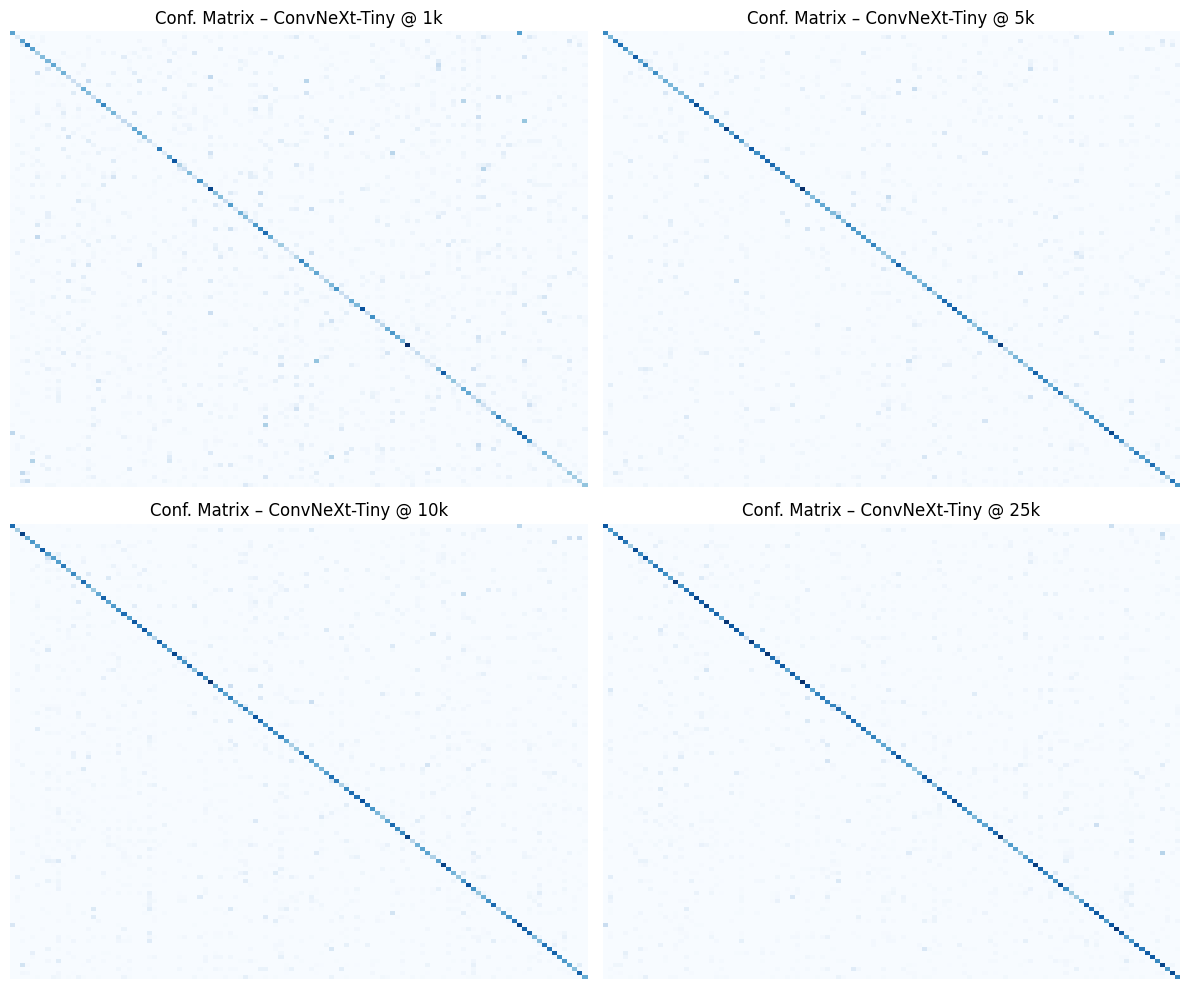
\includegraphics[width=1.0\textwidth]{images/phase03/phase03_ConvNeXt-Tiny_Confusion_Matrix_summary_curve.png}
    \caption{Összehasonlító Confusion Matrix a ConvNeXt-Tiny iteratív tanításáról 10 EPOCH-on keresztül.}
    \label{fig:phase03_ConvNeXt-Tiny_Confusion_Matrix_summary_curve}
  \end{figure}